% Editable native annotations around unchanged verified IDE photographs.
\par
\begin{figure}[htbp]
\centering
\newsavebox{\MARSfirpublishedregistersBox}
\sbox{\MARSfirpublishedregistersBox}{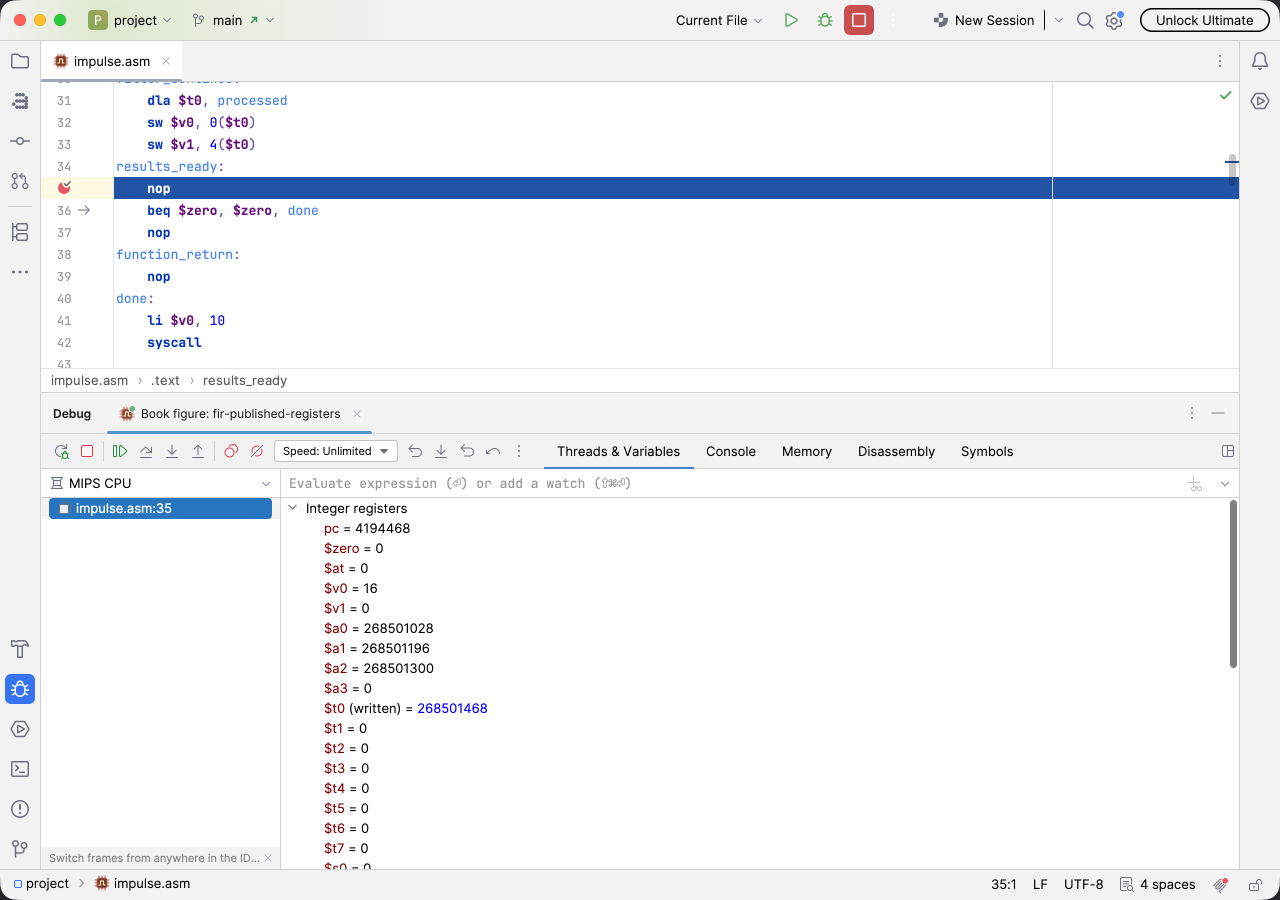
\includegraphics[artifact]{book/captures/021-fixed-point-fir/f02/registers.png}}
\newsavebox{\MARSfirpublishedoutputBox}
\sbox{\MARSfirpublishedoutputBox}{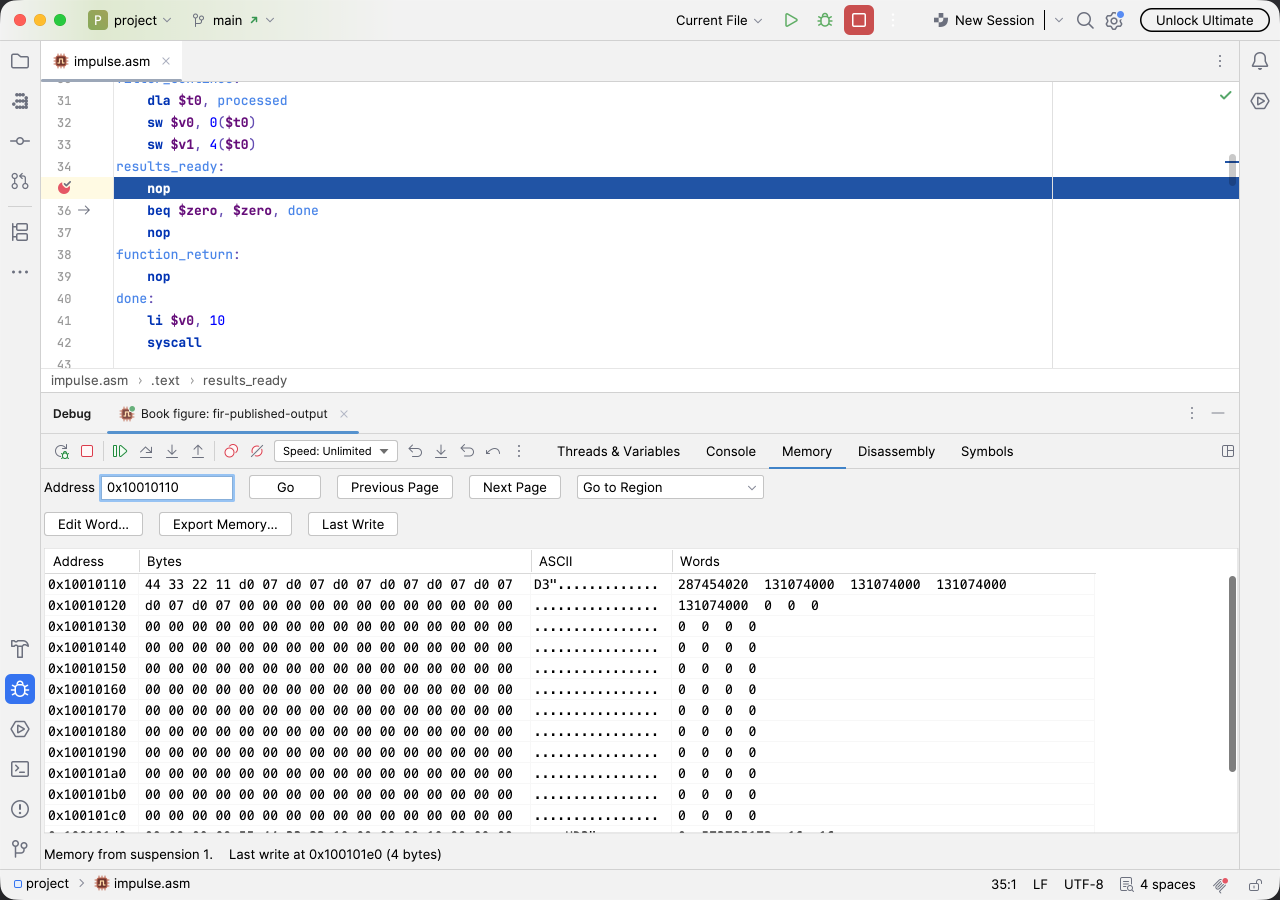
\includegraphics[artifact]{book/captures/021-fixed-point-fir/f02/output.png}}
\newsavebox{\MARSfirpublishedcallerBox}
\sbox{\MARSfirpublishedcallerBox}{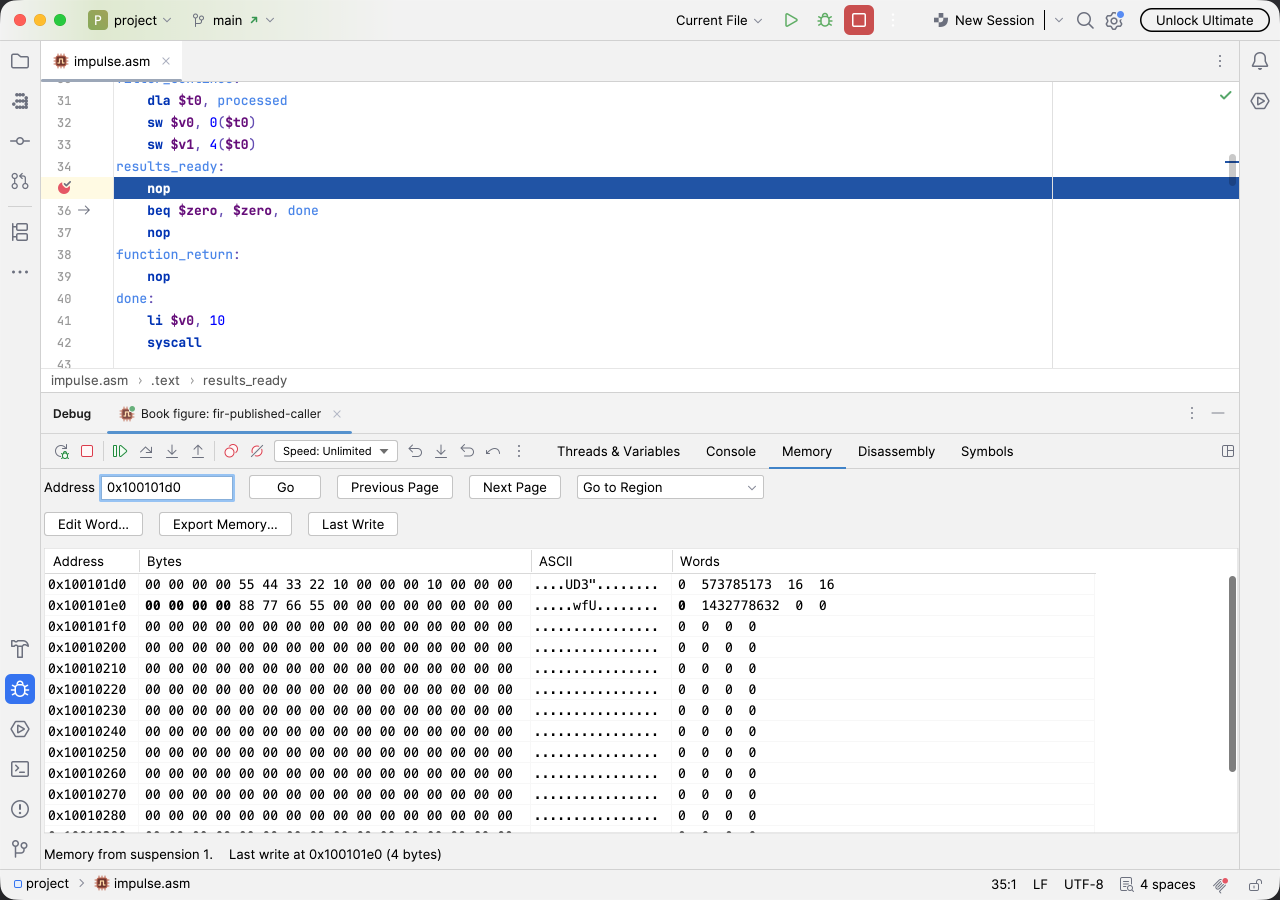
\includegraphics[artifact]{book/captures/021-fixed-point-fir/f02/caller.png}}
\edef\MARSfirpublishedsourceLeft{\the\dimexpr0.036718750\wd\MARSfirpublishedregistersBox\relax}
\edef\MARSfirpublishedsourceBottom{\the\dimexpr0.774444444\ht\MARSfirpublishedregistersBox\relax}
\edef\MARSfirpublishedsourceRight{\the\dimexpr0.713281250\wd\MARSfirpublishedregistersBox\relax}
\edef\MARSfirpublishedsourceTop{\the\dimexpr0.170000000\ht\MARSfirpublishedregistersBox\relax}
\edef\MARSfirpublishedregistersLeft{\the\dimexpr0.246093750\wd\MARSfirpublishedregistersBox\relax}
\edef\MARSfirpublishedregistersBottom{\the\dimexpr0.312222222\ht\MARSfirpublishedregistersBox\relax}
\edef\MARSfirpublishedregistersRight{\the\dimexpr0.553906250\wd\MARSfirpublishedregistersBox\relax}
\edef\MARSfirpublishedregistersTop{\the\dimexpr0.640000000\ht\MARSfirpublishedregistersBox\relax}
\edef\MARSfirpublishedoutputLeft{\the\dimexpr0.034375000\wd\MARSfirpublishedoutputBox\relax}
\edef\MARSfirpublishedoutputBottom{\the\dimexpr0.287777778\ht\MARSfirpublishedoutputBox\relax}
\edef\MARSfirpublishedoutputRight{\the\dimexpr0.584375000\wd\MARSfirpublishedoutputBox\relax}
\edef\MARSfirpublishedoutputTop{\the\dimexpr0.608888889\ht\MARSfirpublishedoutputBox\relax}
\edef\MARSfirpublishedcallerLeft{\the\dimexpr0.034375000\wd\MARSfirpublishedcallerBox\relax}
\edef\MARSfirpublishedcallerBottom{\the\dimexpr0.311111111\ht\MARSfirpublishedcallerBox\relax}
\edef\MARSfirpublishedcallerRight{\the\dimexpr0.584375000\wd\MARSfirpublishedcallerBox\relax}
\edef\MARSfirpublishedcallerTop{\the\dimexpr0.608888889\ht\MARSfirpublishedcallerBox\relax}
\begin{tikzpicture}[alt={Four annotated panels at results_ready show current returns sixteen and zero, all sixteen impulse output halfwords and saved processed/clipped words sixteen and zero. The first eight outputs are 2000 and the remaining eight are zero. Output is a distinct slice from input and coefficients; exit has not executed.}]
\node[anchor=north west,inner sep=0,font=\small\bfseries] (source-title) at (6mm,0) {Next instruction at this boundary};
\node[anchor=north west,inner sep=0] (source) at ([yshift=-1mm]source-title.south west) {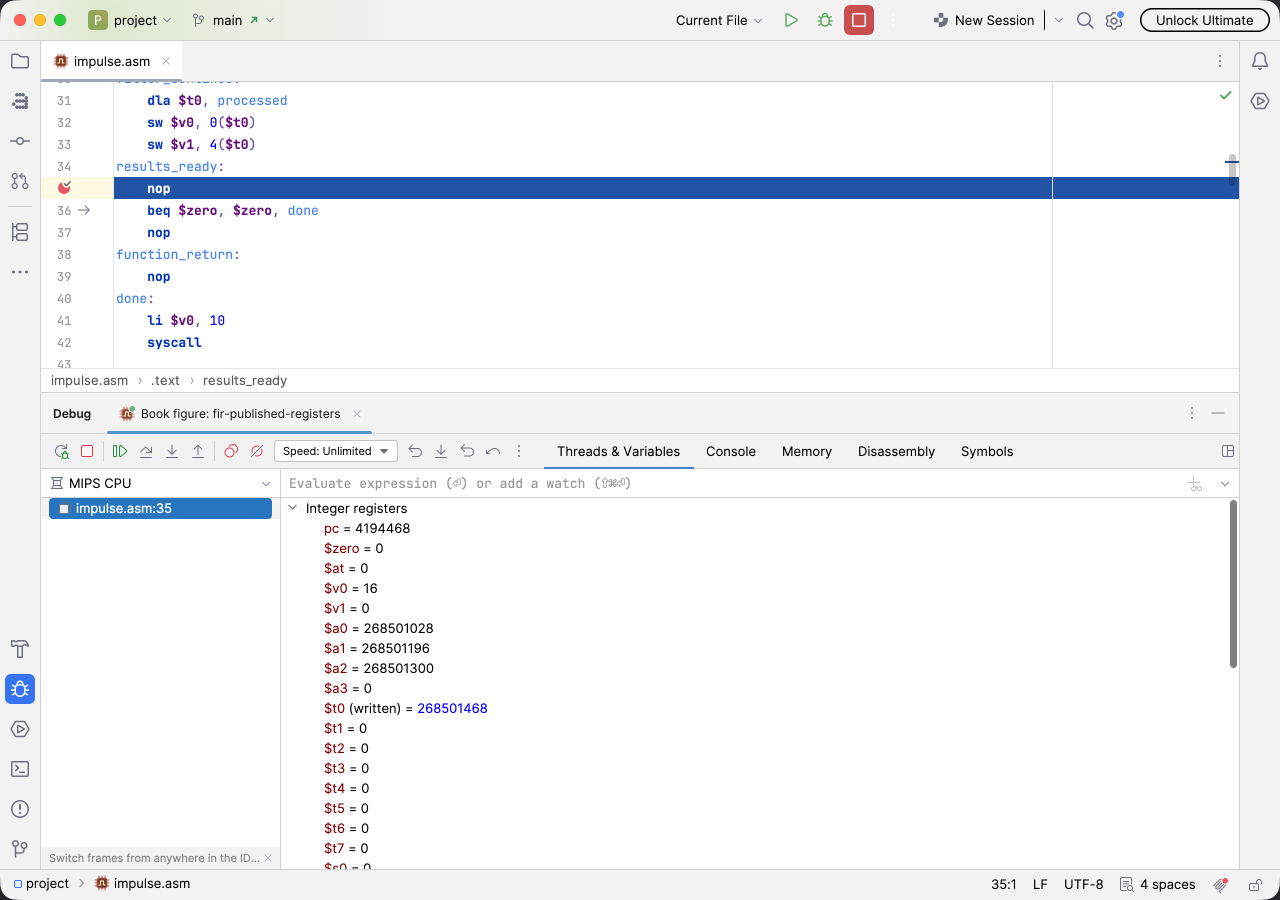
\includegraphics[width=0.54\linewidth,artifact,trim={\MARSfirpublishedsourceLeft{} \MARSfirpublishedsourceBottom{} \MARSfirpublishedsourceRight{} \MARSfirpublishedsourceTop{}},clip]{book/captures/021-fixed-point-fir/f02/registers.png}};
\begin{scope}[shift={(source.south west)},x={($(source.south east)-(source.south west)$)},y={($(source.north west)-(source.south west)$)}]
\draw[black,line width=0.7pt] (0.215625000,0.080000000) rectangle (0.384375000,0.520000000);
\node[draw=black,fill=white,circle,inner sep=1.5pt,font=\footnotesize] at ($(0.215625000,0.520000000)+(-3mm,0)$) {1};
\end{scope}
\node[anchor=north west,inner sep=0,font=\small\bfseries] (registers-title) at (0.58\linewidth,0 |- source-title.north) {Register values at this boundary};
\node[anchor=north west,inner sep=0] (registers) at ([yshift=-1mm]registers-title.south west) {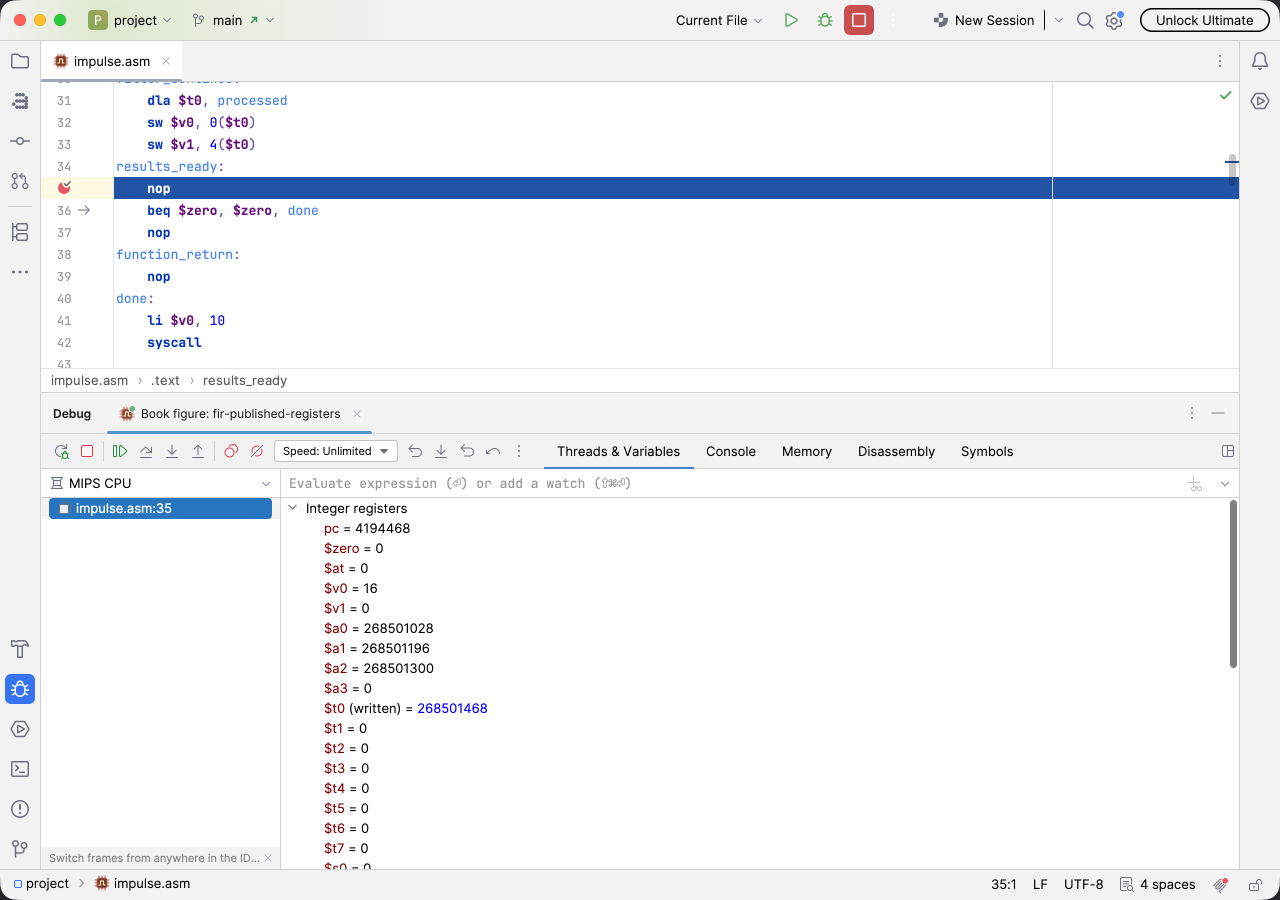
\includegraphics[width=0.42\linewidth,artifact,trim={\MARSfirpublishedregistersLeft{} \MARSfirpublishedregistersBottom{} \MARSfirpublishedregistersRight{} \MARSfirpublishedregistersTop{}},clip]{book/captures/021-fixed-point-fir/f02/registers.png}};
\begin{scope}[shift={(registers.south west)},x={($(registers.south east)-(registers.south west)$)},y={($(registers.north west)-(registers.south west)$)}]
\draw[black,line width=0.7pt] (0.023437500,0.023255814) rectangle (0.250000000,0.953488372);
\node[draw=black,fill=white,circle,inner sep=1.5pt,font=\footnotesize] at ($(0.023437500,0.953488372)+(-3mm,0)$) {2};
\end{scope}
\node[anchor=north west,inner sep=0,font=\small\bfseries] (output-title) at ([yshift=-1mm]source.south west) {Selected output halfwords};
\node[anchor=north west,inner sep=0] (output) at ([yshift=-1mm]output-title.south west) {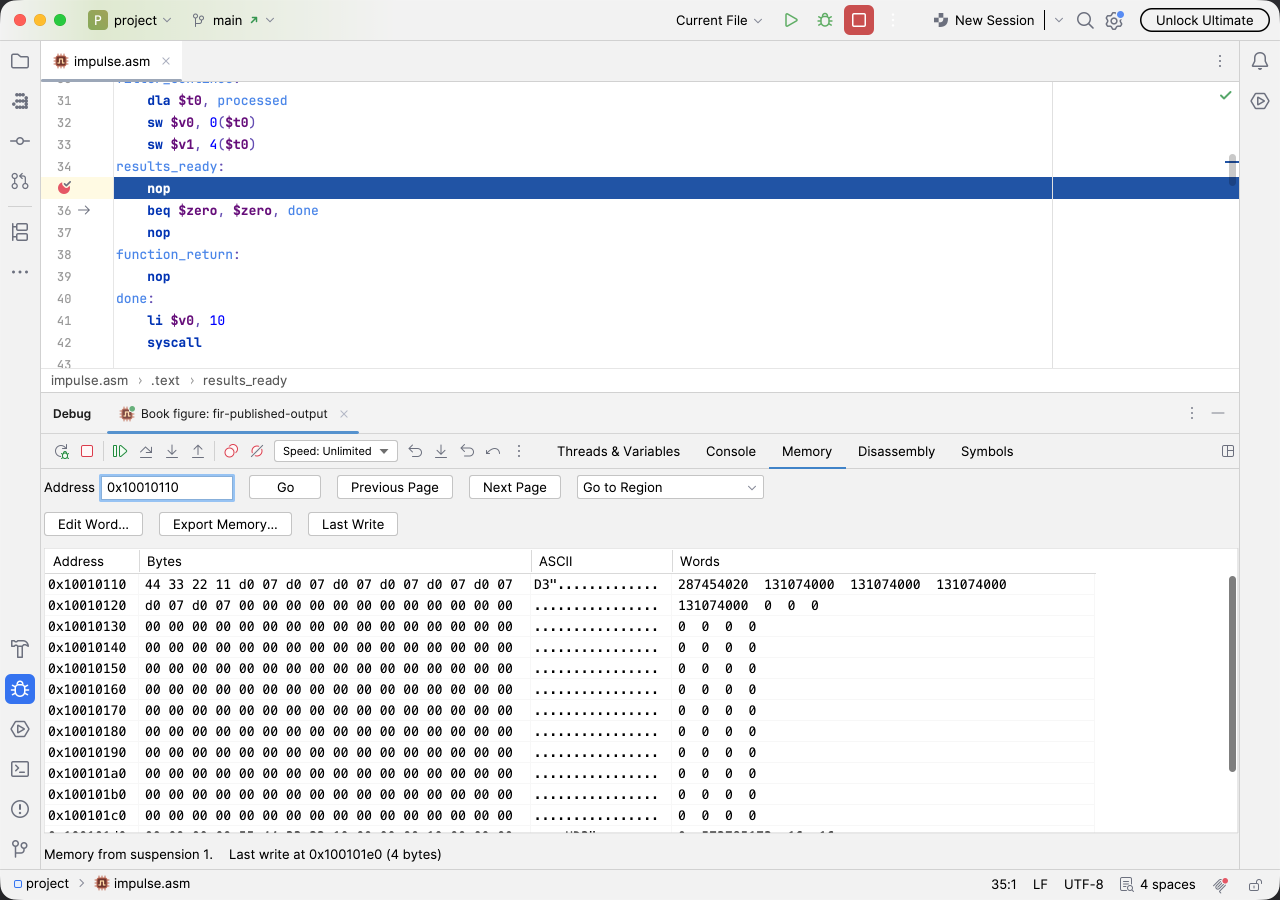
\includegraphics[width=0.84\linewidth,artifact,trim={\MARSfirpublishedoutputLeft{} \MARSfirpublishedoutputBottom{} \MARSfirpublishedoutputRight{} \MARSfirpublishedoutputTop{}},clip]{book/captures/021-fixed-point-fir/f02/output.png}};
\begin{scope}[shift={(output.south west)},x={($(output.south east)-(output.south west)$)},y={($(output.north west)-(output.south west)$)}]
\draw[black,line width=0.7pt] (0.194672131,0.043010753) rectangle (0.997950820,0.720430108);
\node[draw=black,fill=white,circle,inner sep=1.5pt,font=\footnotesize] at ($(0,0.720430108)+(-3mm,0)$) {3};
\end{scope}
\node[anchor=north west,inner sep=0,font=\small\bfseries] (caller-title) at ([yshift=-1mm]output.south west) {Count and saved caller results};
\node[anchor=north west,inner sep=0] (caller) at ([yshift=-1mm]caller-title.south west) {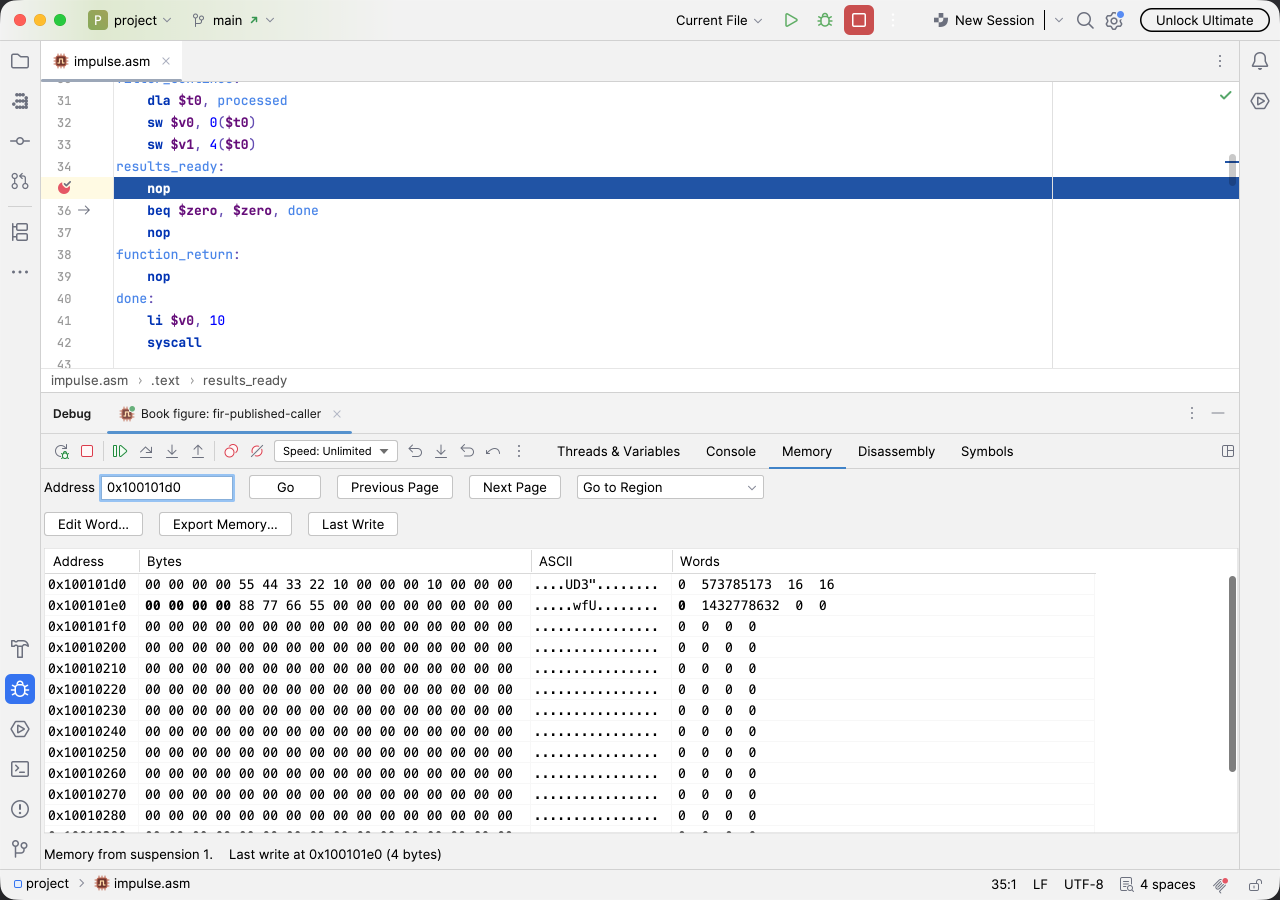
\includegraphics[width=0.84\linewidth,artifact,trim={\MARSfirpublishedcallerLeft{} \MARSfirpublishedcallerBottom{} \MARSfirpublishedcallerRight{} \MARSfirpublishedcallerTop{}},clip]{book/captures/021-fixed-point-fir/f02/caller.png}};
\begin{scope}[shift={(caller.south west)},x={($(caller.south east)-(caller.south west)$)},y={($(caller.north west)-(caller.south west)$)}]
\draw[black,line width=0.7pt] (0.194672131,0.055555556) rectangle (0.997950820,0.638888889);
\node[draw=black,fill=white,circle,inner sep=1.5pt,font=\footnotesize] at ($(0,0.638888889)+(-3mm,0)$) {4};
\end{scope}
\end{tikzpicture}
\par\smallskip
\begin{minipage}{\linewidth}
\small
\begin{enumerate}
\setlength{\itemsep}{2pt}
\setlength{\parsep}{0pt}
\item The blue \texttt{nop} at \texttt{results\_ready} follows both caller stores. The function return and publication are complete; this is a later boundary than \texttt{filter\_ready}, with identical output bytes.
\item The registers still contain \texttt{\$v0 = 16} and \texttt{\$v1 = 0}. Exit later reuses \texttt{v0} for a service number. Inspect the function\textquotesingle s result at the named stop.
\item The 32-byte output slice at \texttt{0x10010114} contains eight halfwords of 2000, then eight of zero. A sliding eight-tap window includes the impulse exactly eight times. Bytes beyond these sixteen outputs remain padding, rather than extra results.
\item The saved \texttt{processed} word at \texttt{0x100101dc} is now 16 and \texttt{clipped} at \texttt{0x100101e0} is zero. The requested count lies immediately before them. Input, coefficients and all guards remain unchanged.
\end{enumerate}
\end{minipage}
\caption{The completed impulse response has eight nonzero outputs and saved counts sixteen and zero.}
\label{capture:021-fixed-point-fir-f02}
\label{fir-f02}
\end{figure}
\par
